\documentclass[11pt]{beamer}
\usetheme{Warsaw}
\usepackage[utf8]{inputenc}
\usepackage[english]{babel}
\usepackage{amsmath}
\usepackage{amsfonts}
\usepackage{amssymb}
\usepackage{graphicx}
\author{Sascha Wernegger}
\title{Multimedia Data Formats}
%\setbeamercovered{transparent} 
%\setbeamertemplate{navigation symbols}{} 
%\logo{} 
%\institute{} 
%\date{} 
%\subject{} 

\newenvironment<>{varblock}[2][.9\textwidth]{%
  \setlength{\textwidth}{#1}
  \begin{actionenv}#3%
    \def\insertblocktitle{#2}%
    \par%
    \usebeamertemplate{block begin}}
  {\par%
    \usebeamertemplate{block end}%
  \end{actionenv}}
\begin{document}

\begin{frame}
\titlepage
\end{frame}

%\begin{frame}
%\tableofcontents
%\end{frame}

\begin{frame}{Compression}
	\begin{itemize}
		\item ImageMagick
		\item JXRLIB
	\end{itemize}
	
\end{frame}

\begin{frame}{Sample}
	\begin{figure}
		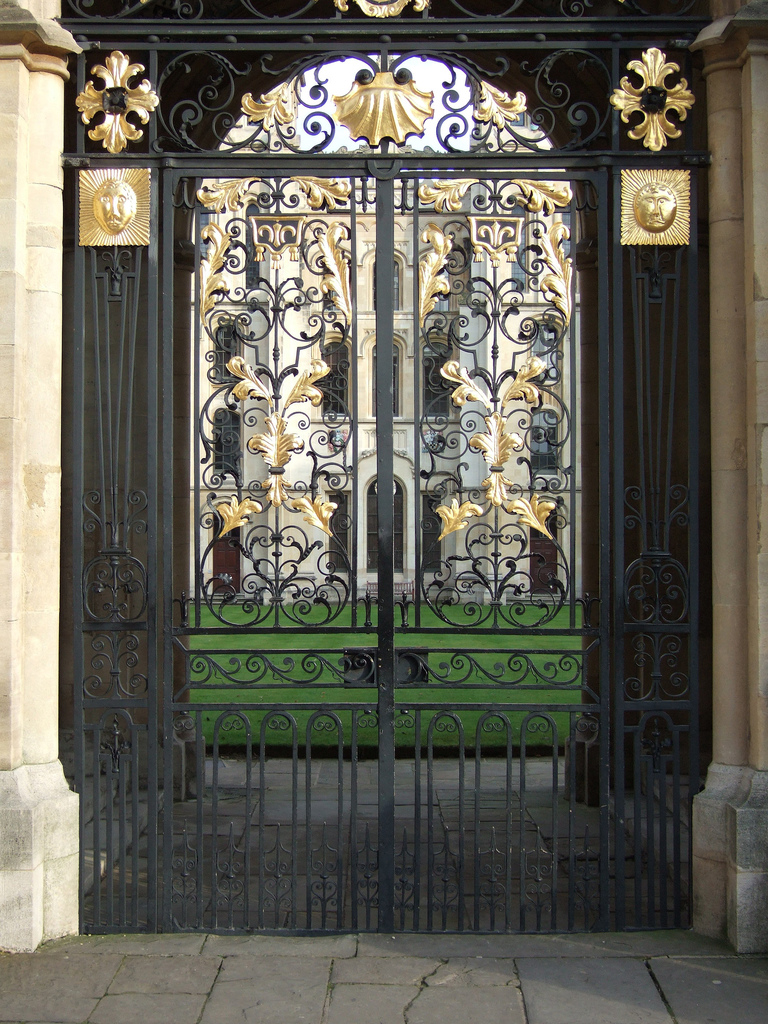
\includegraphics[width=0.5\textwidth]{img/jpg_100.jpg}
	\end{figure}
\end{frame}

\begin{frame}{Comparison}
	\begin{figure}
		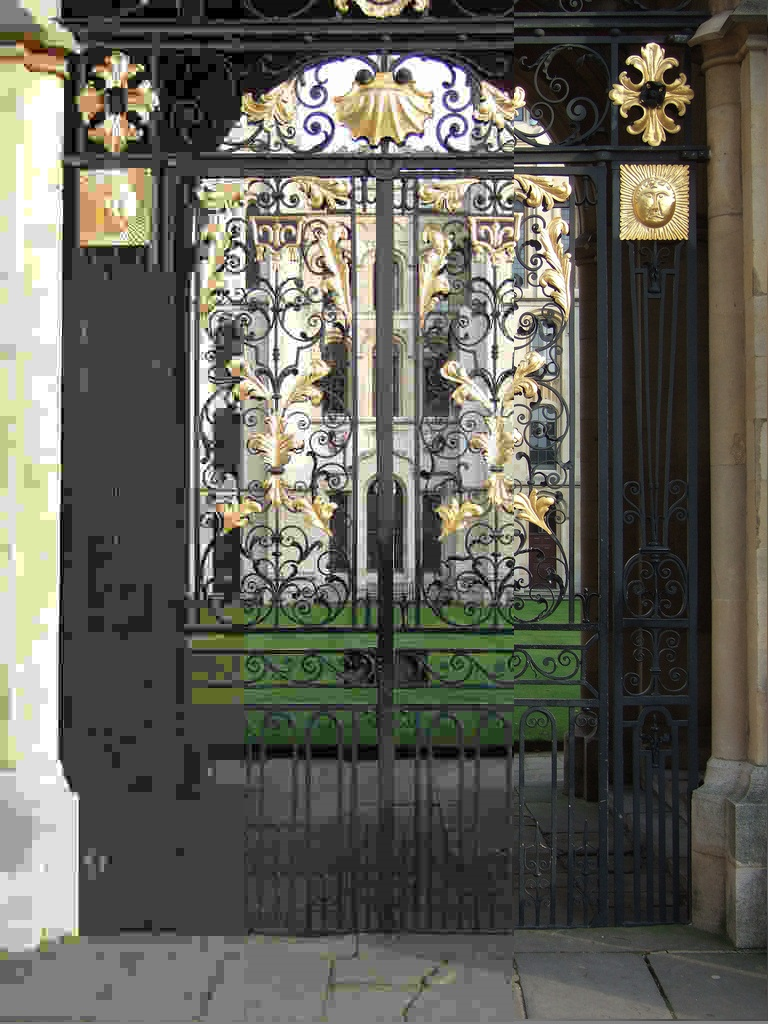
\includegraphics[width=0.35\textwidth]{img/jpg.jpg}
		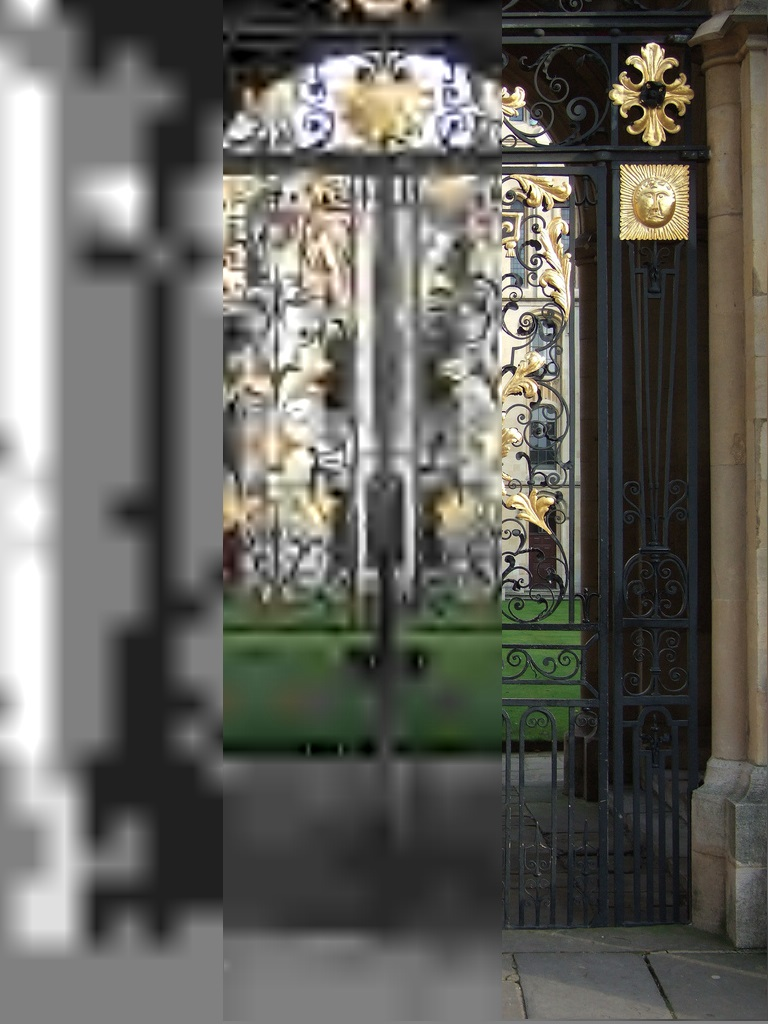
\includegraphics[width=0.35\textwidth]{img/jp2.jpg}
		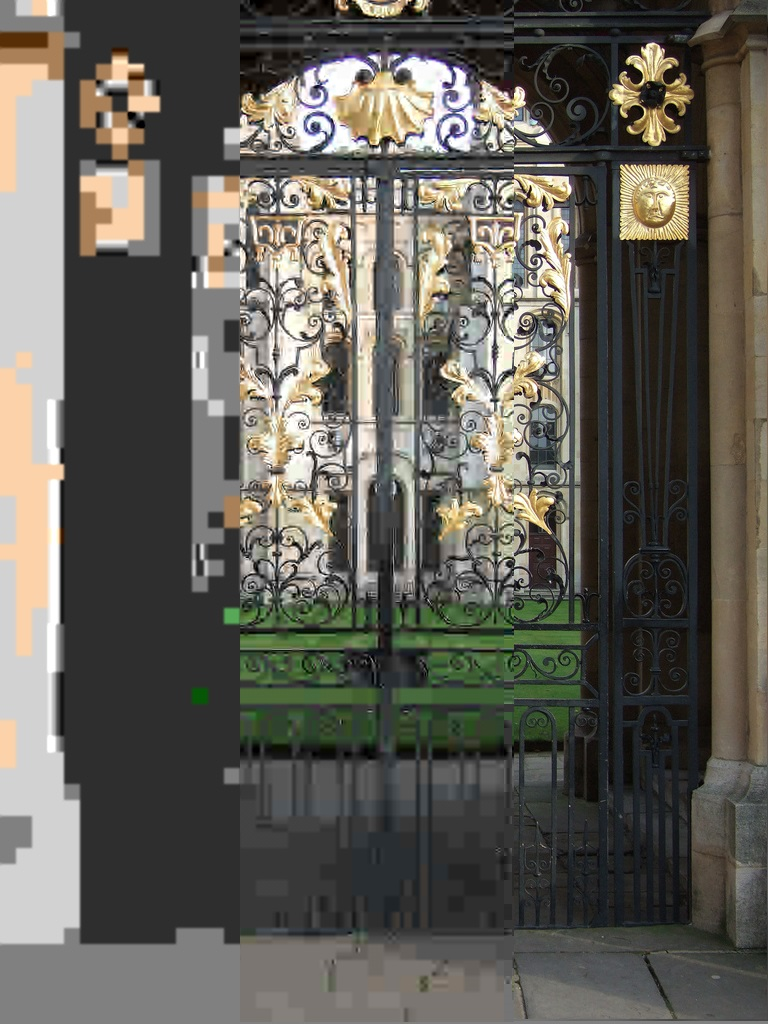
\includegraphics[width=0.35\textwidth]{img/jxr.jpg}
	\end{figure}
\end{frame}

\begin{frame} {Estimate Compression Ratio}
			\begin{block}{t}	
				$s$ : avg size = 391.659 bytes.\\
				$p$ :  avg pixels = 765.969 pixel.\\
				$bpp$ : byte per pixel = 3.\\
				$r$ : avg raw size = $p*bpp$ = 2297908.\\
				$e$ : estimated ratio = $r/s = 5.867$.
			\end{block}	
			\begin{equation}
				\textbf{Estimated Compressionratio = }
			\end{equation}
\end{frame}
\begin{frame}
	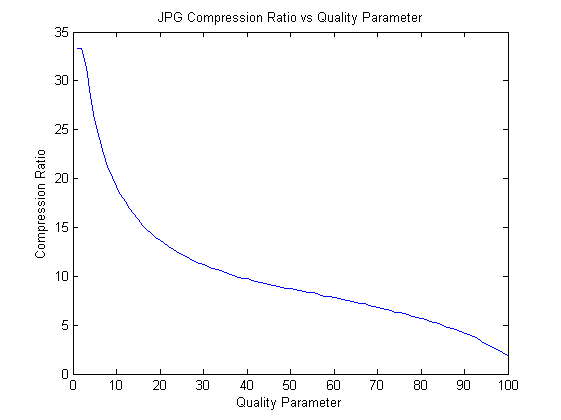
\includegraphics[width=0.8\textwidth]{img/jpg-ratio.png}
\end{frame}

\section{Feature Detectors}
\begin{frame}{FeatureDetectors}
	\begin{itemize}
		\item vlfeat
		\begin{itemize}
			\item SIFT
			\item PHOW(DSIFT)
		\end{itemize}
		\item opencv
		\begin{itemize}
			\item SURF
			\item ORB
		\end{itemize}
	\end{itemize}
\end{frame}

\section{Benchmark}
\begin{frame}{Benchmark}
	\begin{itemize}
		\item VLBENCHMARK
	\end{itemize}
	
\end{frame}

\begin{frame}{Dataset}
\begin{block} {Oxford Buildings Dataset}
	\begin{itemize}
		\item 5062 images
		\item compressed loss-less or with minimal loss in JPEG
		\item collected from Flickr by searching for particular Oxford landmarks
		\item manually annotated to generate ground truth for 11 different landmarks
		\item 5 queries per landmark
		\item total of 55 queries
	\end{itemize}
\end{block}
	Random sampled subsets to limit compression and benchmark speed!
\end{frame}


\begin{frame}{Queries}
	The query consists of a reference image and 4 query sets:
	\begin{itemize}
		\item [good] A nice, clear picture of the object
		\item [ok] More than 25\% of the object is clearly visible.
		\item [junk] Junk Less than 25\% of the object is visible, or there are very high levels of occlusion or distortion.
		\item [bad]  Object not present
	\end{itemize}
	\begin{tabular}{ll}
		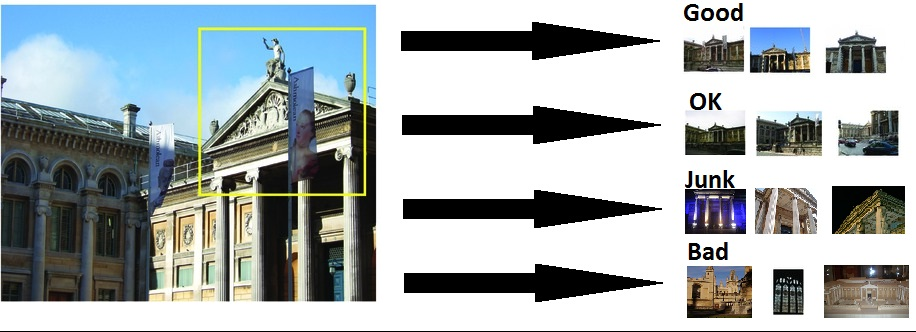
\includegraphics[width=0.7\textwidth]{img/query.jpg}
	\end{tabular}
	now similarity between these image is measured
\end{frame}

\begin{frame} {Generic Local Feature Extractor}
	\begin{block}{Local Feature Frames}
		\begin{itemize}
			\item search image for interest points
			\item define a frame for that point(points,circles,elipses)
		\end{itemize}
	\end{block}	 
	\begin{block}{Descriptor}
		\begin{itemize}
			\item compute descriptor using the frame
		\end{itemize}
	\end{block}
	So we got n frames and n descriptors
\end{frame}

\begin{frame} {Retrieval System}
	\begin{block}{Ranking}
		\begin{itemize}
			\item calculate KNN for the every reference descriptor
			\item vote with descriptor distance for the image
			\item normalize
			\item sort images after voting
		\end{itemize}
	\end{block}
		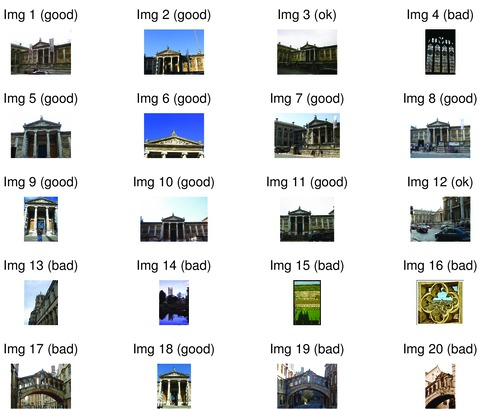
\includegraphics[width=0.5\textwidth]{img/retrieved.jpg}
\end{frame}

\section{Performance Evaluation}

\begin{frame}{Recall Precision}
	\begin{tabular}{ll}

		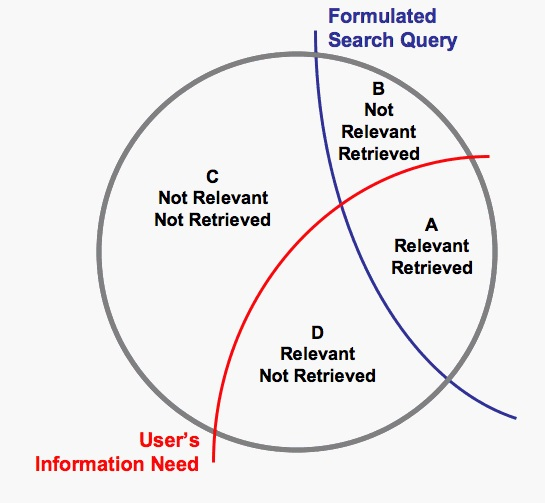
\includegraphics[width=0.5\textwidth]{img/RecallPrecision.jpg}
		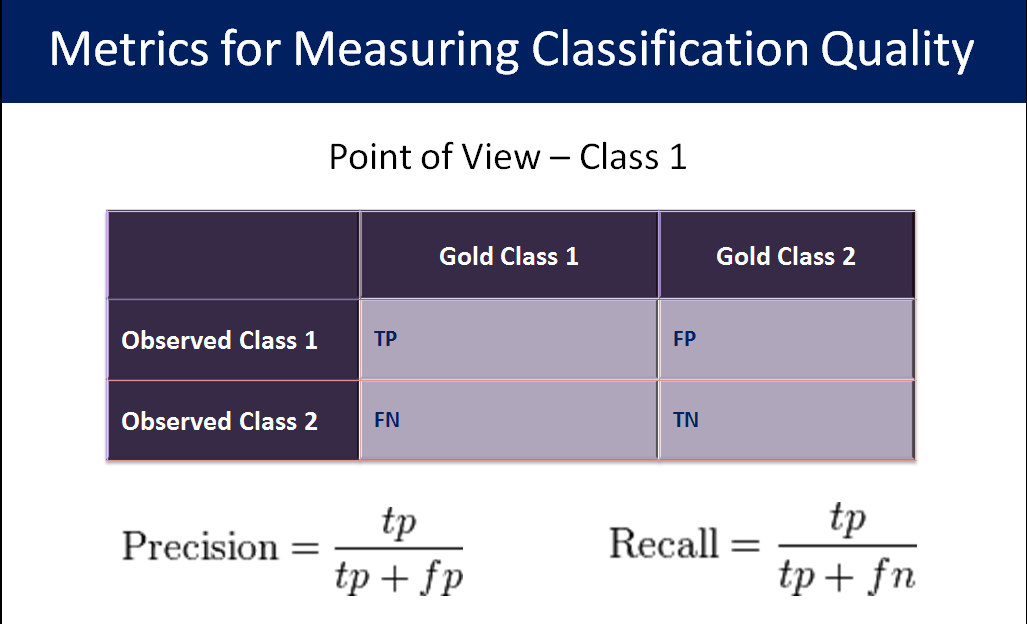
\includegraphics[width=0.5\textwidth]{img/precision_recall.png}

	\end{tabular}

\end{frame}

\begin{frame}{Mean Average Precision}

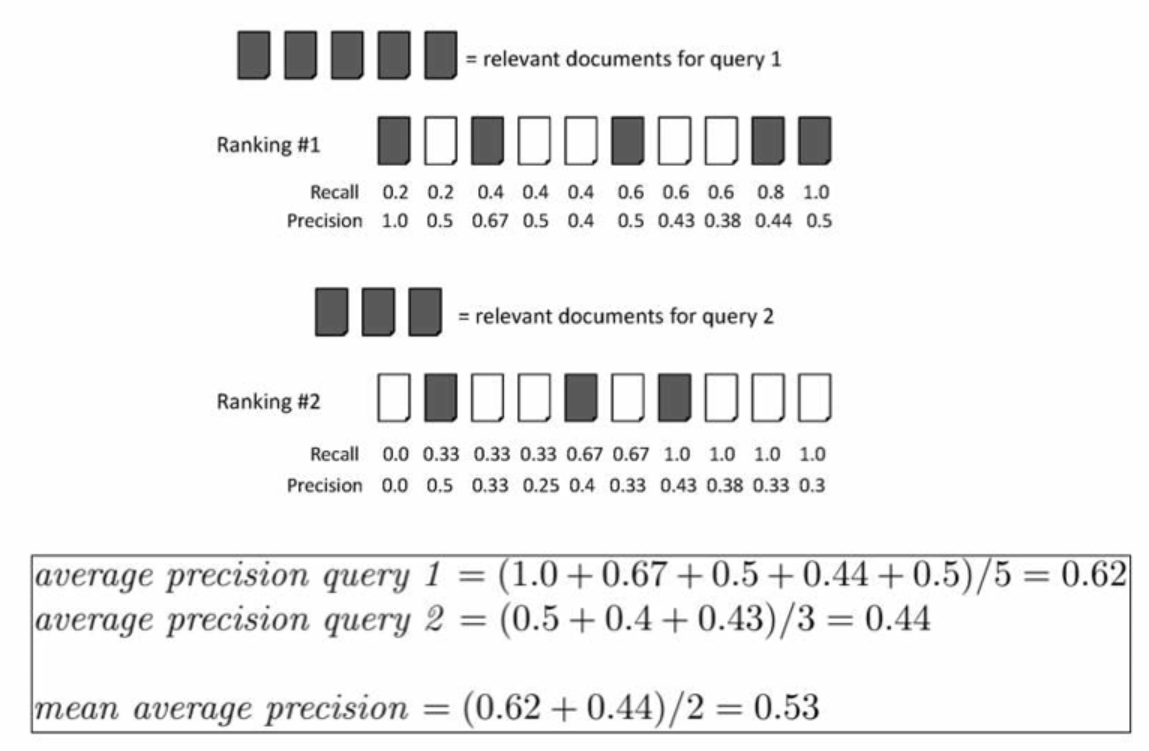
\includegraphics[width=0.9\textwidth]{img/map.png}

\end{frame}

\begin{frame}{Mean Average Precision add}
	\begin{block}{How use the four query classes}
		\begin{itemize}
			\item good and ok images are relevant
			\item junk will be ignored
			\item bad will count as wrong
		\end{itemize}
	\end{block}
\end{frame}

\begin{frame}{Results}
	\begin{itemize}
		\item plot of mAP over image file size
		\item plot query precision
		\item plot prc
	\end{itemize}
\end{frame}

\end{document}
